\documentclass[titlepage, a4paper, openbib, 10pt]{article}

%#####################################
%Usepackages en installingen
\usepackage[top=1in, bottom=1in, left=1in, right=1in]{geometry}
\usepackage[pdftex]{graphicx}
\usepackage{fancyhdr}
\usepackage{sectionbox}
\usepackage[dutch]{babel}
\usepackage{chngcntr}
\usepackage{cite}
\usepackage{url}
\usepackage{makeidx}
\usepackage{paralist}
\usepackage{enumitem}
\usepackage{tocloft}
\usepackage{listliketab}	
\usepackage[table]{xcolor}
\usepackage{tabularx}
\usepackage{epsfig}
\usepackage{pdflscape}
\usepackage{pdfpages}
\usepackage{float}
\usepackage{amsmath}
\usepackage{comment}
\usepackage{multirow} 
\usepackage{rotating}
\usepackage[utf8]{inputenc}
\usepackage{color}
\newcommand{\red}[1]{
\textcolor{red}{#1}
}
\usepackage{verbatim}
\usepackage{listings}
\lstset{language=C,
basicstyle=\ttfamily\footnotesize,
frame=shadowbox,
mathescape=true,
showstringspaces=false,
showspaces=false,
breaklines=true}


%\usepackage{showframe} %tmp
%#####################################
%Nieuwe commando's
\newcommand{\HRule}{\rule{\linewidth}{1pt}}
\newcommand{\organisatie}{\uppercase{Hogeschool Rotterdam / CMI}}
\newcommand{\modulenaam}{Algorithms}
\newcommand{\modulecode}{\uppercase{INFDEV03-6A}}
\newcommand{\stdPunten}{4 ects}
\renewcommand{\author}{G. Costantini}

\definecolor{lichtGrijs}{RGB}{169,169,169}



%#####################################
%Index en styling
\setlength{\cftbeforesecskip}{10pt}
\setlength\parindent{0pt}
\makeindex
\graphicspath{{img}}
\counterwithin{figure}{subsection}
\pagestyle{fancy}
\setcounter{secnumdepth}{5}
\setcounter{tocdepth}{5}

%#####################################
%     Alles voor header/footer
\fancyhf[HL]{\nouppercase{\textit{\leftmark}}}
\setlength{\headheight}{36pt}
\lhead{\uppercase{\footnotesize Course description}}
\chead{\footnotesize \organisatie}
\rhead{
\includegraphics[width=0.09\textwidth]{img/logo}}

\lfoot{\scriptsize \modulenaam}
\cfoot{\scriptsize \today}
\rfoot{\small \thepage}

\renewcommand{\headrulewidth}{0.4pt}
\renewcommand{\footrulewidth}{0.4pt}

\newcommand{\lga}{Analyse the performance of an algorithm [\texttt{PERF}]}
\newcommand{\lgb}{Infer the behavior of algorithms involving basic data structures and analyse their performance [\texttt{DS}\textsuperscript{A}]}
\newcommand{\lgc}{Implement sorting algorithms [\texttt{SORT}\textsuperscript{I}]}
\newcommand{\lgd}{Infer the behavior of sorting algorithms and analyse their performance [\texttt{SORT}\textsuperscript{A}]}
\newcommand{\lge}{Implement recursive data structures [\texttt{REC}\textsuperscript{I}]}
\newcommand{\lgf}{Infer the behavior of algorithms manipulating recursive data structures and analyse their performance [\texttt{REC}\textsuperscript{A}]}
\newcommand{\lgg}{Implement graphs representation and algorithms [\texttt{GRAPH}\textsuperscript{I}]} 
\newcommand{\lgh}{Infer the behavior of algorithms manipulating graphs and analyse their performance [\texttt{GRAPH}\textsuperscript{A}]}			
				 

%#####################################

\begin{document}

%#####################################
%Titlepage
\begin{titlepage}
\thispagestyle{fancy}
\ 
\vspace{5cm}

\begin{center}

	
	\Large \textbf \organisatie
	
	\vspace{1.5cm}
	
	\HRule \\[0.4cm]
	
	\Huge \textbf \modulenaam
	
	\vspace{1.7cm}
	
	\Large \textbf  \modulecode
	
	\vspace{0.4cm}
	
	\HRule \\[1.5cm]
\end{center}
\vfill

% Author and supervisor
\begin{tabular}{l l}
	Number of study points:  & \stdPunten\\
	Course owners: & \author\\
\end{tabular}

\end{titlepage}

%####### Contentpagina ########
%\renewcommand{\baselinestretch}{1.5}\normalsize
%\tableofcontents
%\newpage
%\listoffigures
%\newpage
%\listoftables
%\newpage

%########### Inhoud ###########

\shadowsectionbox
\section*{Module description}
\begin{tabularx}{\textwidth}{|>{\columncolor{lichtGrijs}} p{.26\textwidth}|X|}
	\hline
	\textbf{Module name:} & \modulenaam\\
	\hline
	\textbf{Module code: }& \modulecode\\
	\hline
	\textbf{Study points \newline and hours of effort for full-time students:} & This module gives \stdPunten, in correspondence with 112 hours:
	\begin{itemize}
		\item 3 x 8 hours frontal lecture
		\item the rest is self-study
	\end{itemize} \\
	\hline
	\textbf{Examination:} & Written exam and practical assessment \\
	\hline
	\textbf{Course structure:} & Lectures \\
	\hline
	\textbf{Prerequisite knowledge:} & Object oriented programming \\
	\hline
	\textbf{Learning tools:} & \begin{itemize}
			\item Book: \textit{Introduction to Algorithms}; authors
			C.E. Leiserson, C. Stein, R. Rivest, and T.H. Cormen
			\item Lesson slides (pdf): found on N@tschool
			\item Assignments, to be done at home (pdf): found on N@tschool
		\end{itemize} \\
	\hline
	\textbf{Connected to \newline competences:} & \begin{itemize}
			\item Realisation
			\item Analysis
		\end{itemize} \\
	\hline
	\textbf{Learning objectives:} &
		At the end of the course, the student can:
			\begin{itemize}
				\item \lga
				\item \lgb
				\item \lgc
				\item \lgd
				\item \lge 
				\item \lgf
				\item \lgg
				\item \lgh
			\end{itemize} \\
	\hline

%\end{tabularx}
%\begin{tabularx}{\textwidth}{|>{\columncolor{lichtGrijs}} p{.26\textwidth}|X|}
%	\hline
	\textbf{Course owners:} & \author\\
	\hline
	\textbf{Date:} & \today \\
	\hline
\end{tabularx}
\newpage


\section{General description}
	Designing and manipulating efficient data structures is at the foundation of computer programming. 
	These data structures solve complex problems through well-known, highly difficult techniques that would simply take too long to rediscover for every application. When faced with certain classes of issues, lack of knowledge of algorithms and data structures might significantly impact a programmer's ability to tackle a given problem efficiently and effectively. \\	
	In this course we are going to explain some popular algorithms and data structures used in a variety of scenario's encountered in practice when dealing with structuring and traversal of data. \\

\subsection{Relationship with other teaching units}
	This course builds upon the development courses of the first year.	\\		
		
	Knowledge acquired through the algorithms course is also useful for some of the projects. A word of warning though: projects and development courses are largely independent, so some things that a student learns during the development courses are not used in the projects, some things that a student learns during the development courses are indeed used in the projects, but some things done in the projects are learned within the context of the project and not within the development courses. Moreover, the whole Informatica program is not based on the \textquotedblleft workshop\textquotedblright{} philosophy but rather on building solid foundations preparing students for the future evolutions of computer science (see for instance the module description of Development 1).


\section{Course program}
	
	In the following table you can see the program of the course, divided in lesson units. Each lesson unit is also associated with the corresponding book paragraphs. The last lesson unit of the course is reserved for a summary in preparation for the exam. \\
	Note: Lesson units are intented as collections of topics and do not necessarily correspond to study weeks (for example, a lesson unit could span two study weeks). \\
	
	\begin{tabular}{ | p{1.2cm} | p{10cm} | p{2.7cm} | }
		\hline
	  	\textbf{Lesson unit} & \textbf{Topics} & \textbf{Book chapters and paragraphs} \\
	  	\hline
  		1 & Introduction to algorithms \newline Arrays \newline Complexity of algorithms (empirical analysis, O notation) & 3 \\
  		\hline
  		2 & Sorting algorithms \newline - Insertion sort \newline - Merge sort & 2.1, 2.3 \\
  		\hline
  		3 & List \newline Queue \newline Stack \newline Hash table &  10.1, 10.2, 11.1 until 11.4 \\
  		\hline
  		4 & Trees \newline - BST \newline - k-d trees \newline - 2-3 trees & 12.1 until 12.3, 18 \\
  		\hline
  		5 & Graphs \newline - undirected \newline - directed \newline - Dijkstra's shortest path & 22.1 until 22.3, 24.3 \\
  		\hline
  		6 & Dynamic programming \newline Floyd-Warshall & 15.3, 25.2\\
  		\hline
  		7 & Course review and exam simulation & \\
  		\hline
	\end{tabular}
\begin{comment}
  		4 & Binary search trees & 3.2 \\
  		\hline
  		5 & Balanced search trees: 2-3 search trees & 3.3 \\
  		\hline
  		6 & Graphs (undirected; directed; Dijkstra shortest path) & 4.1, 4.2, 4.4 \\
  		\hline
  		7 & Dynamic programming; Floyd-Warshall & Not covered by the book, see slides or Cormen\\
  		\hline
  		8 & Course recap & \\
  		\hline
\end{comment}


\section{Assessment}
	The course is tested with two exams: a practical assessment and a theoretical examination. The final grade is determined by the practical assessment. However, to be admitted to the practical assessment, you \textbf{must} have a sufficient (i.e. $\geq$ 5.5) grade in the theoretical examination. If your grade in the theoretical examination is not sufficient, then we will register a 0 (zero) in Osiris as grade of the practical assessment.
	
	The correspondence between learning goals and assessment parts is shown in the following table. \\
	
	\begin{table}[h]
		\centering
	\begin{tabular}{ |l|l|l| }
		\hline
		\textbf{Learning goal} & \textbf{Theory} & \textbf{Practice} \\
		\hline
		\texttt{PERF} & V & \\
		\hline 
		\texttt{DS}\textsuperscript{A} & V & \\
		\hline 
		\texttt{SORT}\textsuperscript{I} & & V \\
		\hline 
		\texttt{SORT}\textsuperscript{A} & V & \\
		\hline 
		\texttt{REC}\textsuperscript{I} & & V \\
		\hline 
		\texttt{REC}\textsuperscript{A} & V &  \\
		\hline 
		\texttt{GRAPH}\textsuperscript{I} & & V \\
		\hline 
		\texttt{GRAPH}\textsuperscript{A} & V & \\
		\hline 
	\end{tabular}
	\end{table}

	\subsection{Theoretical examination}
	The theoretical examination consists of a \textbf{written exam} which covers the topics seen in class. The questions will be both theoretical and about code analysis.
	The exam lasts one lesson hour (50 minutes). No help is allowed during the exam.\\
	
	The exam consists of multiple-choice questions about:
	\begin{itemize}
		\item complexity of algorithms (``What is the complexity of the following code/algorithm?")
		\item inference of the behaviour of a given algorithm (for example, ``What does this algorithms do?'' or ``Does this algorithm find the minimum element?'', ``What is the next step of this algorithm given the following state?'' etc.)
		\item definitions given during the course
	\end{itemize}

	\noindent
	Each correct answer is worth 1 point. The grade of the written exam is computed as the percentage of correct answers in a scale from 0 to 10. For example, if the exam is made of 20 questions and you answer correctly 14 questions, then your grade is 14 * 10 / 20 = 7.

	\subsection{Practical assessment}
	The practical examination is a \textbf{practical assessment} during which the student is asked to implement (completely or in part) algorithms seen during the course or strictly connected to course topics. The practical assessment consists of a few assignments asking to fill in code of given partially-implemented algorithms.
	
	The programming language used for the practical assessment will be C\#. You need to install Visual Studio on your laptop before the practical assessment.
	
	As preparation for the assessment, the students are strongly suggested to complete a \textbf{formative programming assignment} (see Attachment 2). In this programming assignment, some of the data structures and algorithms seen in class will have to be implemented and applied to a specific case study.

	
	\subsection{Retake (herkansing)}
	If one part of the assessment is not sufficient (theoretical and/or practical examination), then you can repeat that part in the following educational period:
	\begin{itemize}
	\item In week 10 of the following OP you can repeat the written exam.
	\item In week 10 of the following OP you can repeat the practical assessment (if the written exam has been already passed).
	\end{itemize}
	


%\bibliographystyle{plain}
%\bibliography{references}
%\newpage
%\section*{Attachment 1: Written exam template}
The general shape of a written exam for this course is made up of a series of highly structured open questions.

\paragraph*{Question I: complexity} \ \\

\textbf{General shape of the question:} \textit{Given the following code, what is its (tightest) complexity class using the big-Oh notation?} \ 

\textbf{Grading:} \textit{2 points for correct answer, 0 otherwise.} \ 

\textbf{Associated learning goals:} \texttt{PERF}.

\ \\ 
\paragraph*{Question II: basic data structures (list, queue, stack, hash tables)} \ \\

\textbf{General shape of the question:} \textit{Complete the code below so that it produces the desired result on the specified basic data structure.} \ 

\textbf{Grading:} \textit{2 points for correct answer, 1 point for minor mistakes, 0 otherwise.} \ 

\textbf{Associated learning goals:} \texttt{DS}\textsuperscript{A}.

\ \\ 
\paragraph*{Question III: sorting} \ \\

\textbf{General shape of the question:} \textit{What is the output of the following algorithm if input is ... ? What is the (tightest) complexity class of the algorithm (using the big-Oh notation)?} \ 

\textbf{Grading:} \textit{2 points for correct complexity and output, 1 point for either correct complexity or output, 0 otherwise.} \ 

\textbf{Associated learning goals:} \texttt{SORT}\textsuperscript{A}.

\ \\ 
\paragraph*{Question IV: trees} \ \\

\textbf{General shape of the question:} \textit{Complete the code below so that it produces the desired result (for example, insertion, lookup, traversal, ...) on a tree.} \ 

\textbf{Grading:} \textit{2 points for correct answer, 1 point for minor mistakes, 0 otherwise.} \ 

\textbf{Associated learning goals:} \texttt{REC}\textsuperscript{A}.

\ \\ 
\paragraph*{Question V: graphs} \ \\

\textbf{General shape of the question:} \textit{What does the following algorithm produce? What is the (tightest) complexity class of the algorithm (using the big-Oh notation)?} \ 

\textbf{Grading:} \textit{2 points for correct complexity and output, 1 point for either correct complexity or output, 0 otherwise.} \ 

\textbf{Associated learning goals:} \texttt{GRAPH}\textsuperscript{A}.

\ \\ 



%%%%%%%%%%%%%%%%%%%%%%%%%%%%%%%%%%%%%%%%%

\begin{comment}
	\begin{tabular}{|p{3cm}|p{3.5cm}|p{6cm}|}
		\hline
		\textbf{Learning goal} & \textbf{Dublin descriptors} & \textbf{Tested through} \\
		\hline
		\texttt{KNOW} & 1 & Theoretical examination \\
		\hline
		\texttt{IMPL} & 2 & Practical examination \\
		\hline
		\texttt{AN} & 3 & Theoretical examination \\
		\hline
		\texttt{APP} & 2, 3 & Theoretical and practical examination \\
		\hline
	\end{tabular}
	
	\vspace{1cm}

	Dublin-descriptors:
	\begin{enumerate}
		\item Knowledge and understanding
		\item Applying knowledge and understanding
		\item Making judgements
		\item Communication
		\item Learning skills
	\end{enumerate}
\end{comment}
%\newpage
%/\include{tex/Practicums}
%/\newpage
%/\section*{Exam structure}
What follows is the general structure of a DEV5 exam.
\\ 
\\
\textbf{Associated learning goals:} \texttt{ORM}, \texttt{RDBMS}.
\textbf{Points:} \textit{25\%.}
\paragraph{Question I: SQL queries} \ \\

\textit{Given a database definition writes the SQL code for the requested queries} 

\ \\


\textbf{Answer:} \textit{}

\begin{lstlisting}
\end{lstlisting}


\ \\ 
\textbf{Associated learning goals:} \texttt{OPT}, \texttt{RDBMS}.
\textbf{Points:} \textit{25\%.}
\paragraph{Question II: Query optimization in SQL} \ \\ 

\textit{Given the following queries identify at least N-columns to be indexed with suitable index}

\begin{lstlisting}
\end{lstlisting}

\ \\ 

\textbf{Associated learning goals:} \texttt{TRANS-CONS}, \texttt{RDBMS}.
\textbf{Points:} \textit{25\%.}
\paragraph{Question III: Transaction management and concurrency}

\ \\ 

\textit{Given the following N-queries, which are run in parallel, show plausible solutions }
\begin{lstlisting}
\end{lstlisting}

\ \\ 

\textbf{Answer:} \textit{...}


\ \\ 
\textbf{Associated learning goals:} \texttt{NON-REL}.
\textbf{Points:} \textit{25\%.}
\paragraph{Question IV: Crash recovery}

\ \\ 

\textit{Given the following log file explain the behaviour of the crash recovery and the UNDO/DO phases}

\begin{lstlisting}
\end{lstlisting}

\ \\ 
\textbf{Associated learning goals:} \texttt{NON-REL}.
\textbf{Points:} \textit{25\%.}
\paragraph{Question V: NoSQL databases en Graph Theory}

\ \\ 

\textit{Transoform this relational data model into a graph model OR given this un-/directed graph identify the adjancy list or matrix of it}

\begin{lstlisting}
\end{lstlisting}

\ \\ 

\textbf{Concrete example of answer:} \textit{}

\ \\ 
\textbf{Grading:} \textit{All values are correct: full-points. At least half the values are correct: half points. Zero points otherwise.}

\ \\ 

%/\newpage
%\section*{Exam sample}
What follows is a concrete example of the exam.


\paragraph{Question I: formal rules} \ \\

\textit{You start at point (0,0). Take a step in the direction (10,0) until you are above point (45,0). Then take five steps in the direction (0,2). Where do you end up?}

\ \\ 

\textbf{Answer:} \textit{The trajectory is:}

\begin{lstlisting}

P1 = (50,0)
 +----- P2 = (50,10)
 |
 |
 |
 |
P0 = (0,0)
\end{lstlisting}

\ \\ 

\textbf{Points:} \textit{25\%.}

\ \\ 
\ \\ 

\paragraph{Question II: program state} \ \\ 

\textit{Fill-in the program state with the values that the variables assume while running the sample below.}

\begin{lstlisting}
y = 1
for i in range(0, 5):
    y = y * 2
\end{lstlisting}

\ \\ 

\textbf{Answer:} \textit{The variable allocations are:}

\begin{tabular}{| c | c | c | c | c | c | c | c |}
\hline
\textbf{y} & 1 & 1 & 2 & 4 & 8 & 16 & 32 \\
\hline
\textbf{i} & n.a. & 0 & 1 & 2 & 3 & 4 & 4 \\
\hline
\end{tabular}

\ \\
s
\textbf{Points:} \textit{25\%.}

\ \\ 

\textbf{Grading:} \textit{Full points if all values are correctly listed in the right order. Half points if at least half of values are listed in the right order. Zero points otherwise.}

\ \\ 

\textbf{Associated learning goals:} \texttt{CMC}.

\ \\ 

\paragraph{Question III: variables, expressions, and data types}

\ \\ 

\textit{What is the value and the type of all variables after execution of the following code?}
\begin{lstlisting}
v = 0
i = "Hello + world"
j = "Hello" + "world"
k = 10 / 3
\end{lstlisting}

\ \\ 

\textbf{Answer:} \textit{The value and type of all variables after execution is:}

\begin{tabular}{| l | c | c | }
\hline
\textbf{Variable} & \textbf{Value} & \textbf{Type} \\
\hline
v & 0 & int \\
\hline
i & 'Hello + world' & str \\
\hline
j & 'Helloworld' & str \\
\hline
k & 3 & int \\
\hline
l & 3.3333$\dots$ & float \\
\hline
\end{tabular}

\ \\ 

\textbf{Points:} \textit{25\%.}

\ \\ 

\textbf{Grading:} \textit{All values and types are correct: full-points. At least half the values and at least half the types are correct: half points. Zero points otherwise.}

\ \\ 

\textbf{Associated learning goals:} \texttt{VAR}, \texttt{EXPR}.

\ \\ 

\paragraph{Question IV: control flow}

\ \\ 

\textbf{General shape of the question:} \textit{What is the value of all variables after execution of the following code?}

\ \\ 

\textbf{Concrete example of question:} \textit{What is the value of all variables after execution of the following code?}

\begin{lstlisting}
v = 0
for i in range(1,15):
  if (i % 2 == 0) & (i % 3 == 0):
    v = v + i
\end{lstlisting}

\ \\ 

\textbf{Concrete example of answer:} \textit{The value of all variables after execution is:}

\begin{tabular}{| l | c |}
\hline
\textbf{Variable} & \textbf{Value} \\
\hline
\texttt{i} & \texttt{14} \\
\hline
\texttt{v} & \texttt{18} \\
\hline
\end{tabular}

\ \\ 

\textbf{Points:} \textit{25\%.}

\ \\ 

\textbf{Grading:} \textit{All values are correct: full-points. At least half the values are correct: half points. Zero points otherwise.}

\ \\ 

\textbf{Associated learning goals:} \texttt{COND}, \texttt{LOOP}.

\ \\ 

%##############################

%\section*{Attachment 2: Examination matrix}



\begin{itemize}[noitemsep]
	\item Module: INFDEV03-6A (Algorithms)
	\item Module responsible: G. Costantini
	\item Study points: 4
	\item Exam form: Written exam [W.E.] (prerequisite) + Assessment [A] (100\% final grade)
	\item Exam date: OP 2
\end{itemize}

\begin{table}[!h]
\small
\begin{tabular}{ |p{3cm}|l|l|l|l|r|l|l r| }
\hline
\textbf{Learning goals} & Knowledge & Insight & Apply & Analyse & Synthesize & Evaluate & \multicolumn{2}{l}{Total points}\\
 & & & & [W.E.] & [A] & & [W.E] & [A] \\
\hline
1 \lga & & & & 20\% & & & 20\% &  \\ 
\hline
2 \lgb & & & & 20\% & & & 20\% &  \\ 
\hline
3 \lgc & & & & & 30\% & & & 30\%  \\ 
\hline
4 \lgd & & & & 20\% & & & 20\% &  \\ 
\hline
5 \lge & & & & & 30\% & &  & 30\% \\ 
\hline
6 \lgf & & & & 20\% & & & 20\% &  \\ 
\hline
7 \lgg & & & & & 40\% & &  & 40\% \\ 
\hline
8 \lgh & & & & 20\% & & & 20\% &  \\
\hline
Total points: & & & & 100\% = prereq & 100\% & & 100\% & 100\% \\
\hline
Cesure: & \multicolumn{8}{|p{13cm}|}{Cesure of written exam: 5.5, which is prerequisite to be admitted to the assessment. Cesure is there also 5.5. The student receives a grade only for the assessment.} \\
\hline
Retake: & \multicolumn{8}{|p{13cm}|}{For both written exam and assessment there is a retake (within the scholastic year).}\\
\hline
\end{tabular}
\end{table}
\normalsize

\begin{comment}
\begin{figure}[!h]
	\centering
	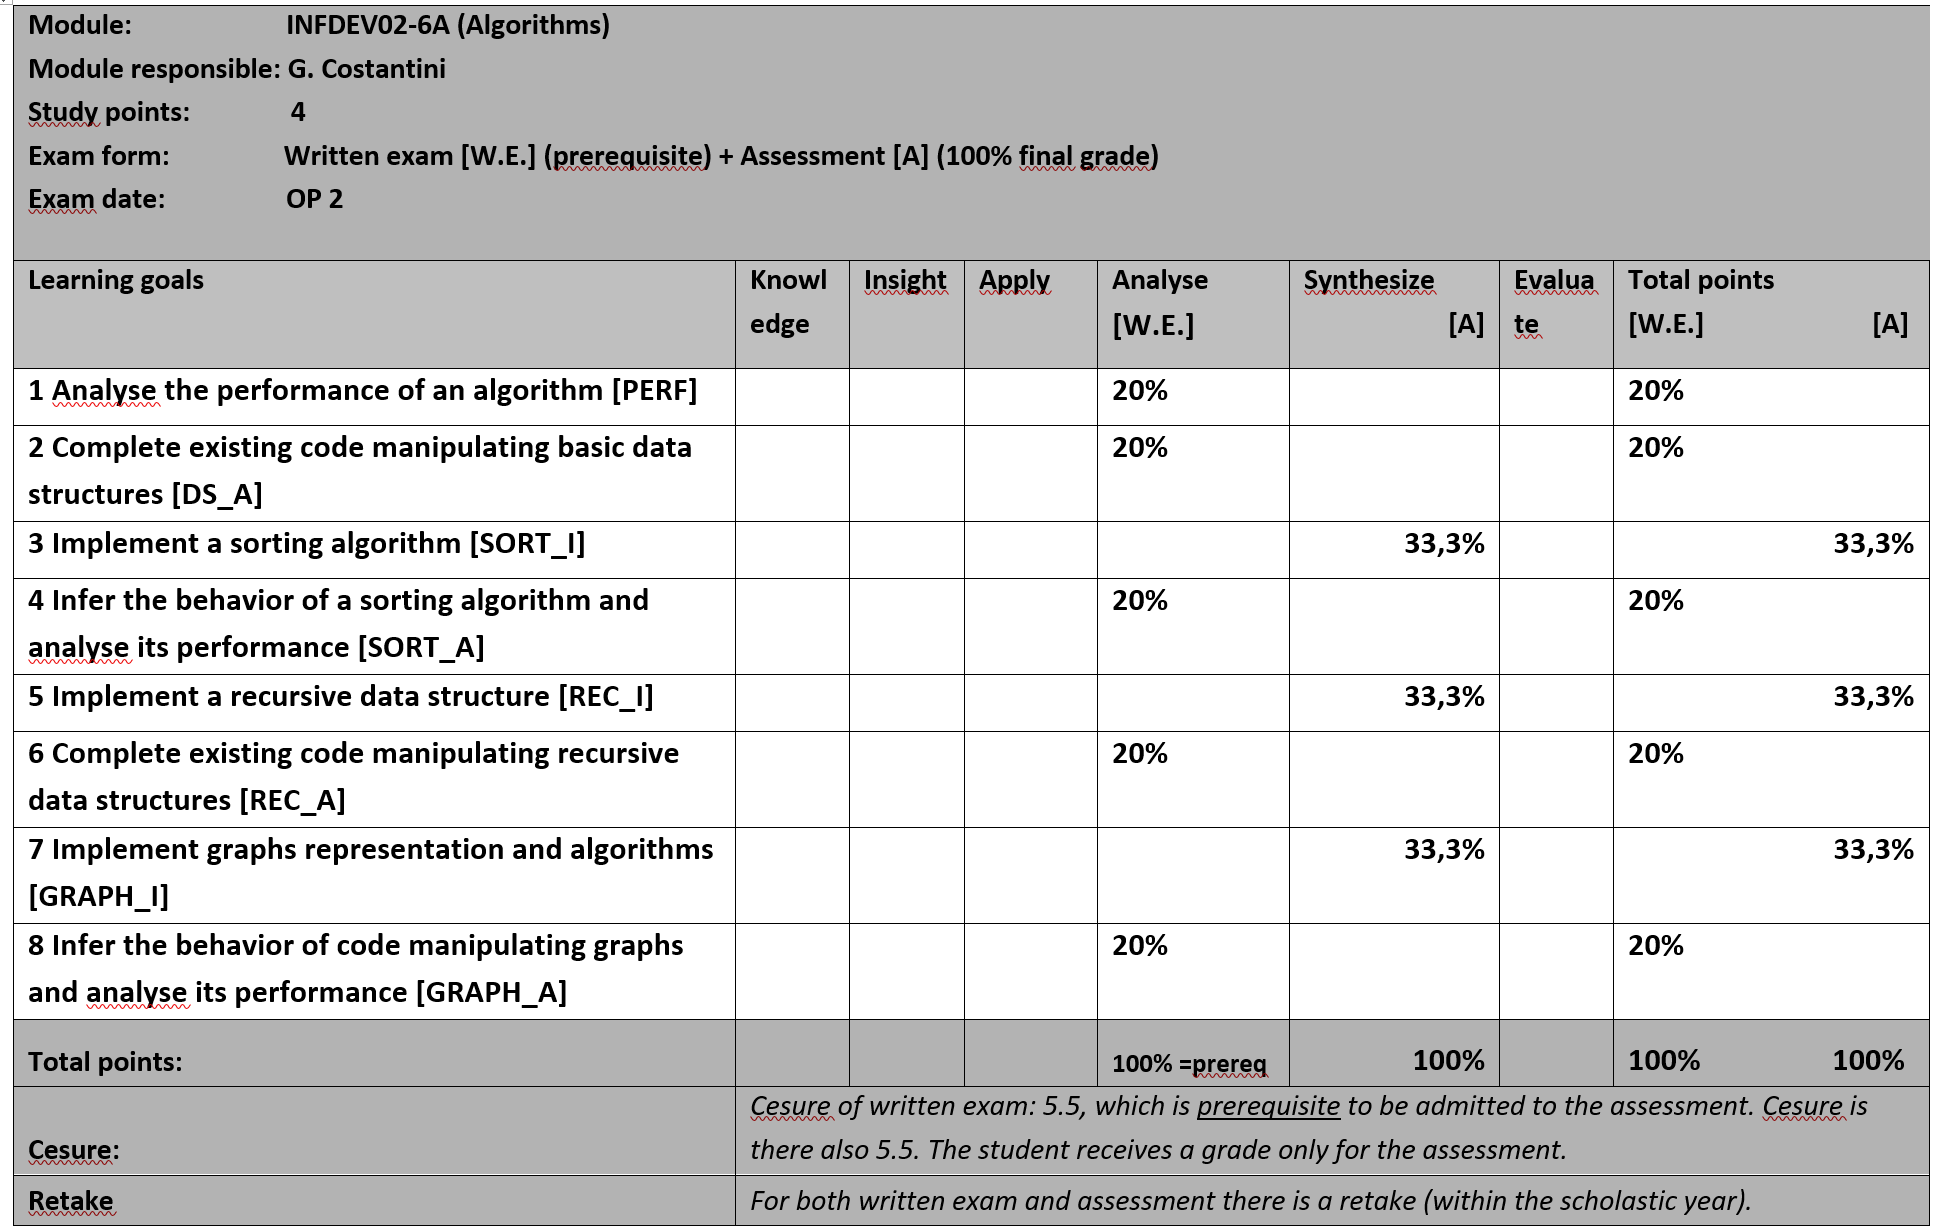
\includegraphics[scale=0.6]{img/toetsmatrijs}
	\caption{Examination matrix of the course}
	\label{img:Ex1}
\end{figure}
\end{comment}

\begin{comment}
\section*{Bijlage 3: Studielast normering in ects}

		Dit hoofdstuk bevat de beschrijving van de procedures om voor beoordeling in aanmerking te komen.\\
		Bijvoorbeeld voldoende aanwezigheid, 80\% van de opdrachten hebben ingeleverd, presentaties hebben verricht etc.\\

		Verder wordt zo gedetailleerd mogelijk beschreven hoe er tot een cijfer wordt gekomen en welke rollen er door docenten en ander betrokkenen hierbij vervuld worden. \\

		Geef een verantwoording van de toets; wat wordt getoetst, waarom is voor deze vorm gekozen.\\

		Vul een toetsmatrijs in voor de toets (zie bijlage).\\

		Beschrijf ook duidelijk de \textbf{herkansingsmogelijkheden}. \\

		Neem in geval van een schriftelijk tentamen een voorbeeldtoets op als bijlage.\\
		Geef daarbij per deelvraag het aantal te verdienen punten aan. \\

		Bij een schriftelijk rapport. Geef de beoordelingscriteria aan met daarbij de mogelijke score en de onderlinge weging. \\

		Toetsduur: \\

		Hoe en wanneer krijgt de student feedback?\\
\end{comment}
%\newpage
\section*{Attachment 1: Practical examination}

\subsection*{General (important) information}
\begin{itemize}
\item The assignment must be implemented using C\# or F\#.
\item The only library tools you are allowed to use are: arrays, lists, and math functions. Other data structures or functions on data structures covered by the course must be implemented \textbf{by hand}.
\end{itemize}

\subsection*{Introduction to the framework}
The exercises will be based on the simulation of a city, containing houses and special buildings (represented through ancient civilization temples), all connected by streets. The student must implement algorithms to answer some queries on the simulated city.
To set up the framework, follow these instructions:

\begin{itemize}
\item Download and install the latest version of Visual Studio Community (\url{https://www.visualstudio.com/en-us/downloads/download-visual-studio-vs.aspx}); choose ``F\# language" during \textit{custom setup}; 
\item Download the project framework from N@tschool (or Github) and open the .sln file; if it is not already set, right click on \texttt{EntryPoint} project (in the solution explorer) and select ``Set as startup project";
\item The functions you have to program are contained in the file \texttt{Program.cs}; for now there are stub versions of the function implementations that you have to replace with yours;
\item Compile the project in debug mode and run it with Ctrl+F5;
\item A window opens asking you which assignment you want to execute: choose a number between 1 and 4 \footnote{In the application, assignment 3 corresponds to exercise 3.1; assignment 4 corresponds to exercise 3.2.} (or q if you want to close it) and press Ok;
\item The simulation will start. You can move the visual with WASD and zoom with Z (zoom in) and X (zoom out).
\item Exit with ESC. 
\end{itemize}

\newpage
\subsection*{Exercise 1 - Sorting}
\textbf{Learning goal}: \texttt{SORT}\textsuperscript{I}. \\

\subsubsection*{Goal}
Sort all special buildings by Euclidean distance from a specified house. The Euclidean distance formula is:
\begin{align*}
d(house,building) = \sqrt{(x_{house} - x_{building})^{2} + (y_{house} - y_{building})^{2} } 
\end{align*}
This means that the connection through roads is not relevant in this exercise (everyone has his private helicopter to move around the city).

\subsubsection*{Function signature} 
\begin{lstlisting}
private static IEnumerable<Vector2> SortSpecialBuildingsByDistance(Vector2 house, IEnumerable<Vector2> specialBuildings)
\end{lstlisting}

This function takes as input a house position (\texttt{Vector2 house}) and a list of building positions (\\ \texttt{IEnumerable<Vector2> specialBuildings}) and returns a sorted list of building positions according to their distance from the house position (\texttt{IEnumerable<Vector2>}). Use the \textbf{merge sort} as sorting algorithm. Any implementation not using this technique will not be accepted and evaluated.\\

\subsubsection*{Result}
As you can see from Figure \ref{img:Ex1}, the selected house is highlighted and there is a number above each special building indicating its position in the sorted list of buildings. 

\begin{figure}[!h]
\centering
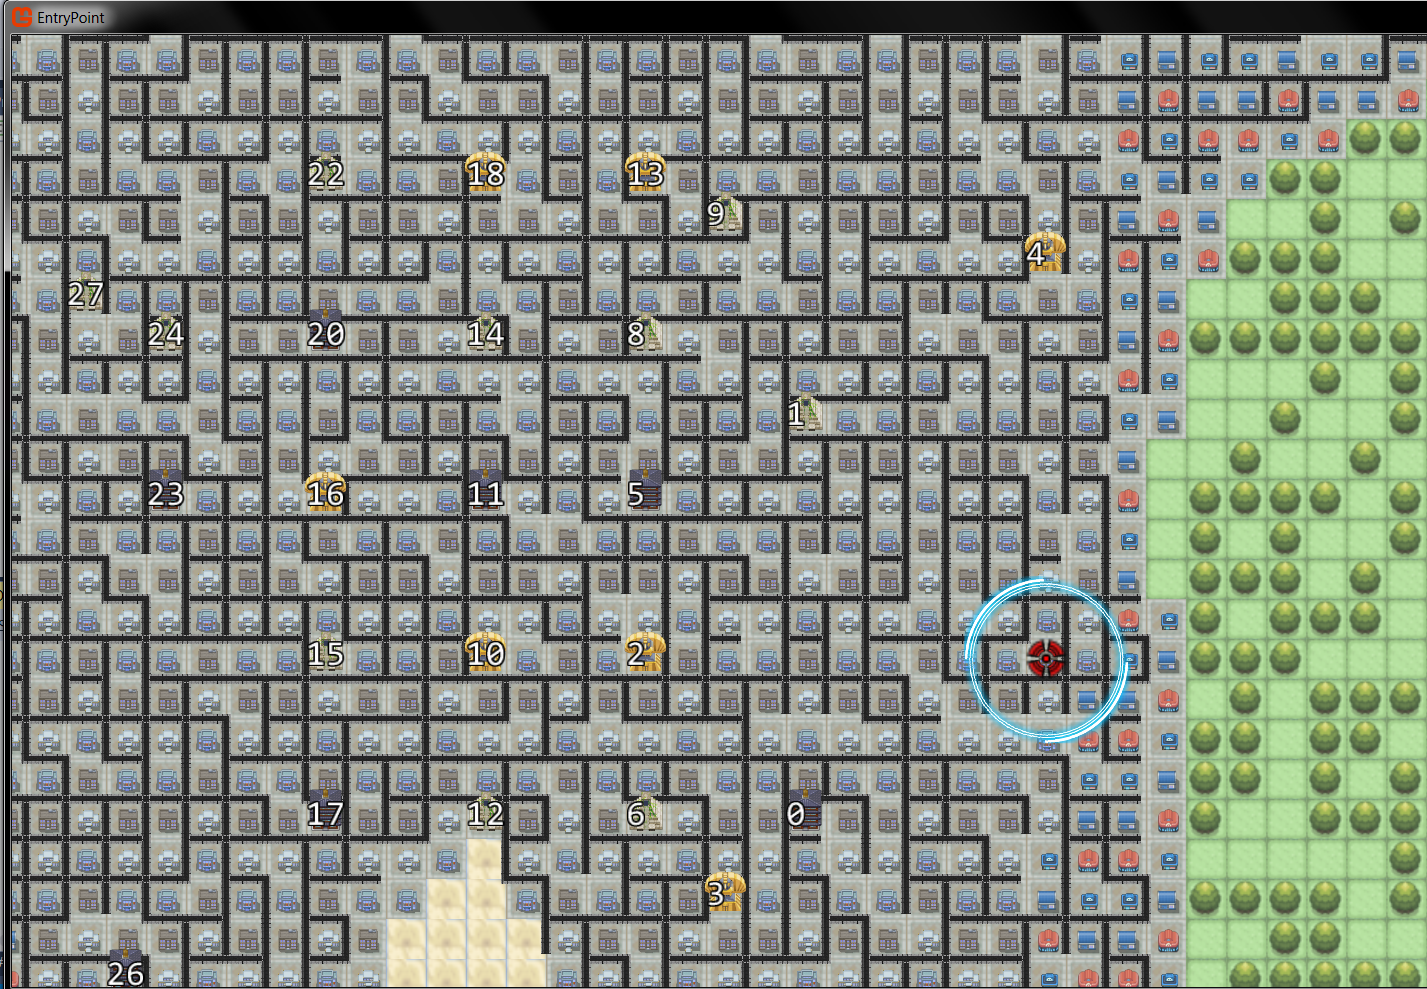
\includegraphics[scale=0.25]{img/exercise1}
\caption{Exercise 1 result}
\label{img:Ex1}
\end{figure}

\newpage
\subsection*{Exercise 2 - Trees}
\textbf{Learning goal}: \texttt{REC}\textsuperscript{I}. \\

\subsubsection*{Goal}
Find all the special buildings within a specified distance from each house. Create a \textbf{k-d tree} to organize the special buildings positions in advance (like explained in class). Then look up the tree for each of the requested houses (with the associated distance).

\subsubsection*{Function signature} 
\begin{lstlisting}
private static IEnumerable<IEnumerable<Vector2>> FindSpecialBuildingsWithinDistanceFromHouse(IEnumerable<Vector2> specialBuildings, IEnumerable<Tuple<Vector2, float>> houseAndDistances)
\end{lstlisting}

\noindent
This function takes as input a list of special building positions (\texttt{IEnumerable<Vector2> specialBuildings}), a list of pairs made of a house position and the maximum distance for a special building to be selected (\texttt{IEnumerable<Tuple<Vector2, float>> houseAndDistances}), and returns a list of lists of positions (\\ \texttt{IEnumerable<IEnumerable<Vector2>>}) of selected special buildings (one list for each house).\\

\subsubsection*{Result}
As you can see from Figure \ref{img:Ex2}, each selected house is surrounded by a circle that should contain all the special buildings within the distance associated to such house. The buildings you return are highlighted in blue, the houses in red.

\begin{figure}[!h]
\centering
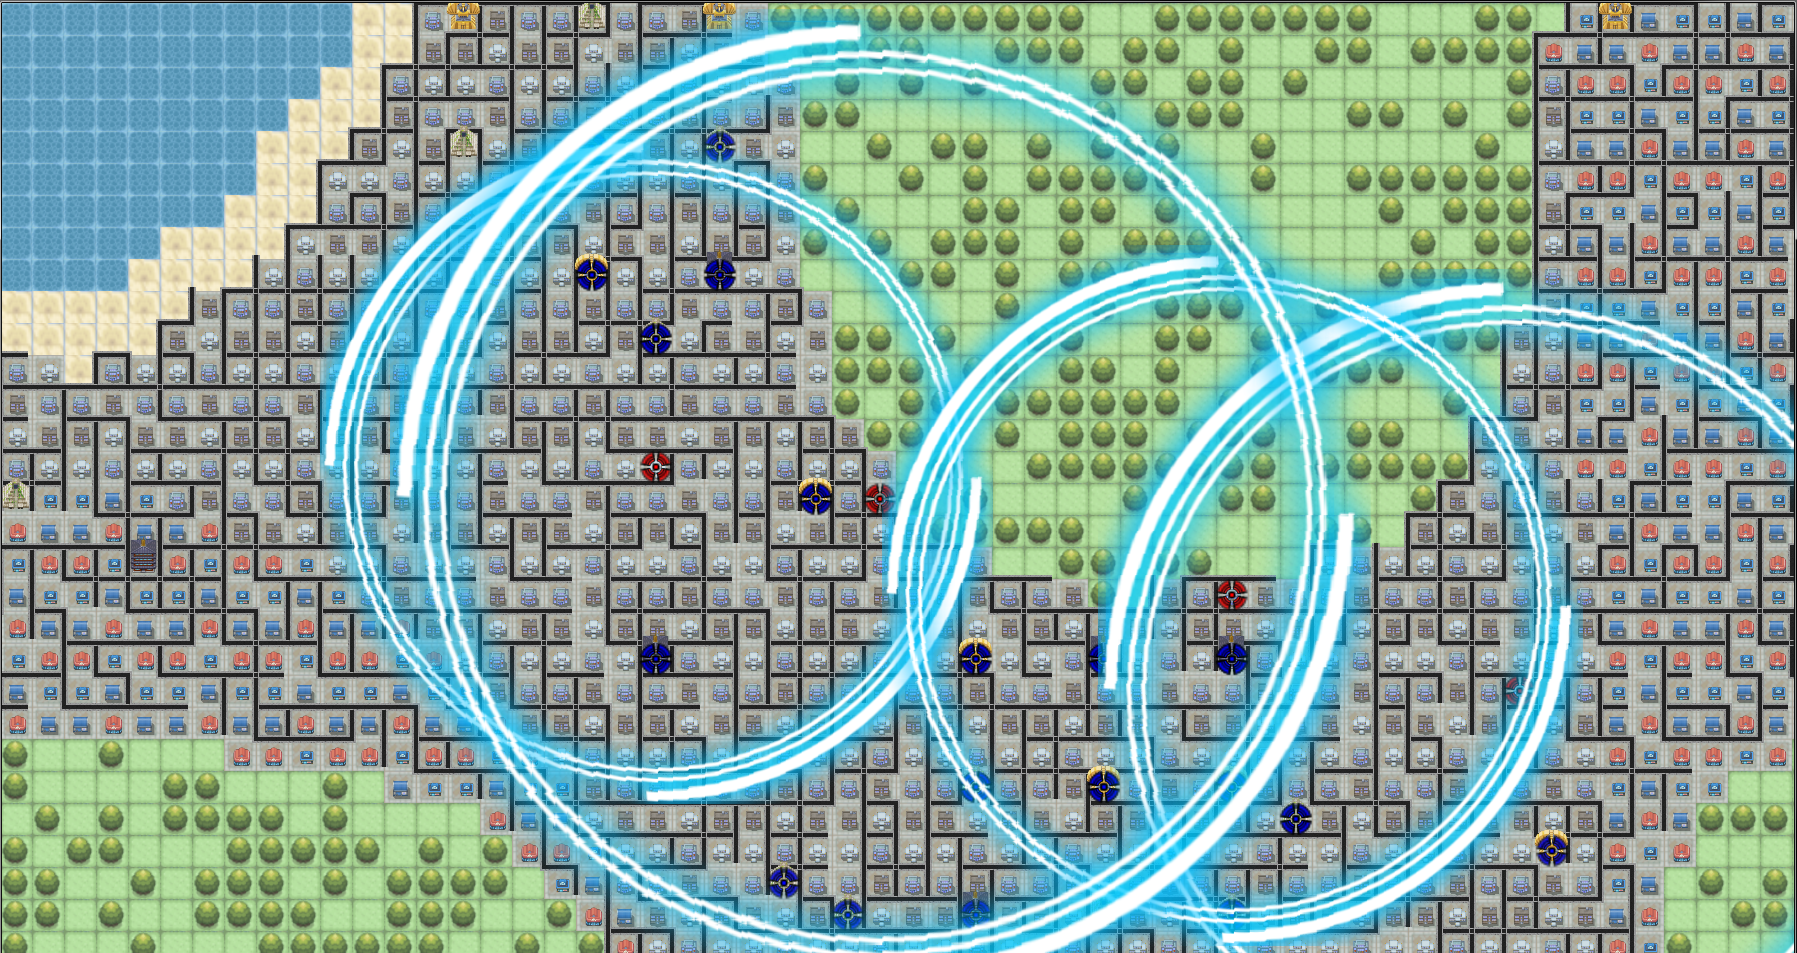
\includegraphics[scale=0.25]{img/exercise2}
\caption{Exercise 2 result}
\label{img:Ex2}
\end{figure}

\newpage
\subsection*{Exercise 3 - Graphs}
\textbf{Learning goal}: \texttt{GRAPH}\textsuperscript{I}. \\

\subsubsection*{Goal}
Find the shortest path(s) from a specified house to other special building(s). The shortest path is made of the road sections to use in order to drive from the house to the special building.\\
\textbf{Remark}: This assignment can be solved in two ways, that is using Dijkstra or Floyd Warshall.\\
\textbf{Hint:} In both assignments, you have to build the adjacency matrix using the starting point and endpoint of the road sections. The weight of the edge is the distance between the two points.

\subsection*{Option 1: Dijkstra}
In this assignment we want to compute the minimum path between one house and one special building. 

\subsubsection*{Function signature} 
\begin{lstlisting}
private static IEnumerable<Tuple<Vector2, Vector2>> FindRoute(Vector2 startingBuilding, Vector2 destinationBuilding, IEnumerable<Tuple<Vector2, Vector2>> roads)
\end{lstlisting}

\noindent
This function takes as input the position of the house to start from (\texttt{Vector2 startingBuilding}), the position of the destination (\texttt{Vector2 destinationBuilding}), and a list of road sections, each represented as a pair of starting point and endpoint (\texttt{IEnumerable<Tuple<Vector2, Vector2>> roads}), and returns a list of road sections (\texttt{IEnumerable<Tuple<Vector2, Vector2>>}) forming the shortest path between the house and the destination.\\

\subsubsection*{Result} 
As you can see from Figure \ref{img:Ex3-1}, the house is surrounded by a circle and highlighted in red. The path to the destination is highlighted with coloured dots.

\begin{figure}[!h]
\centering
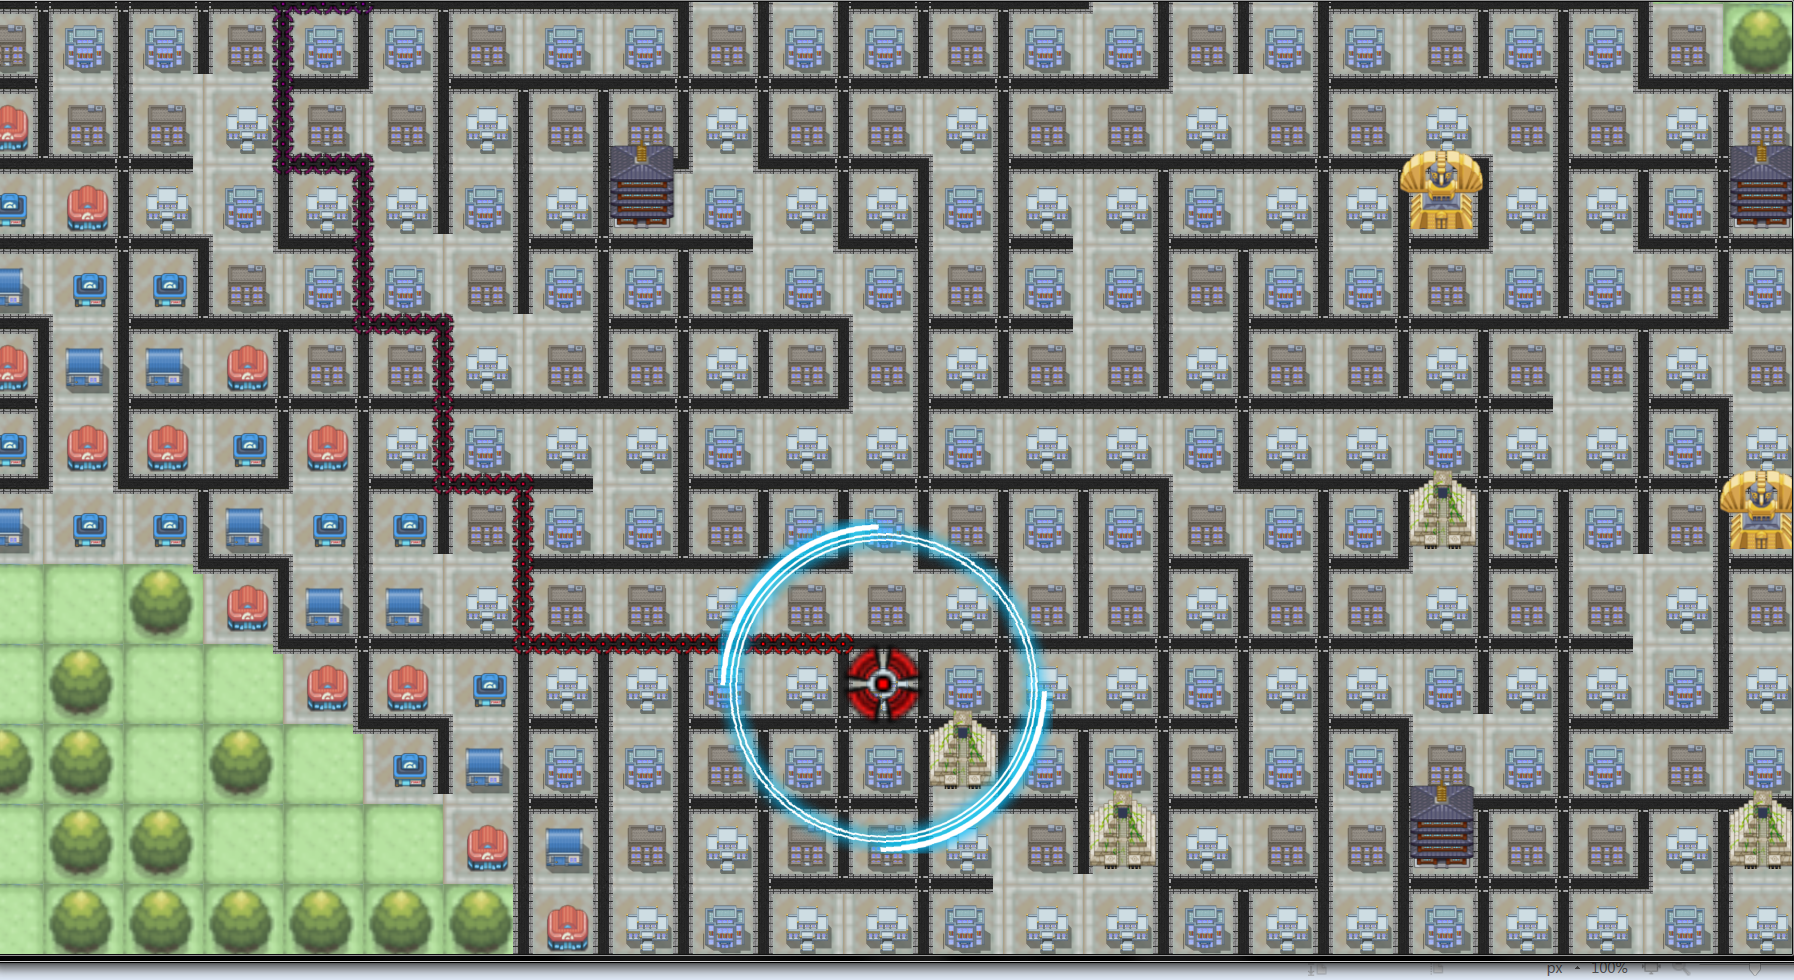
\includegraphics[scale=0.2]{img/exercise3}
\caption{Exercise 3.1 result}
\label{img:Ex3-1}
\end{figure}


\subsection*{Option 2: Floyd Warshall}
In this assignment we want to compute the minimum paths between one house and a list of special buildings. 

\subsection*{Function signature} 
\begin{lstlisting}
private static IEnumerable<IEnumerable<Tuple<Vector2, Vector2>>> FindRoutesToAll(Vector2 startingBuilding, IEnumerable<Vector2> destinationBuildings, IEnumerable<Tuple<Vector2, Vector2>> roads)
\end{lstlisting}

\noindent
This function takes as input the position of the house to start from (\texttt{Vector2 startingBuilding}), the positions of all the destinations (\texttt{IEnumerable<Vector2> destinationBuildings}), and a list of road sections, each represented as a pair of starting point and endpoint (\texttt{IEnumerable<Tuple<Vector2, Vector2>> roads}), and returns a list of shortest paths (\texttt{IEnumerable<IEnumerable<Tuple<Vector2, Vector2>>>}). Each shortest path is referred to one specific destination and is made of a list of road sections.
The function must precompute the all-pairs shortest path with Floyd Warshall algorithm and then extract only the paths requested by the function from the distance and predecessor matrices.\\

\subsection*{Result}
As you can see from Figure \ref{img:Ex3-2}, the house is surrounded by a circle and highlighted in red. The destinations are highlighted in blue. The paths from the house to all destinations are highlighted with coloured dots.

\begin{figure}
\centering
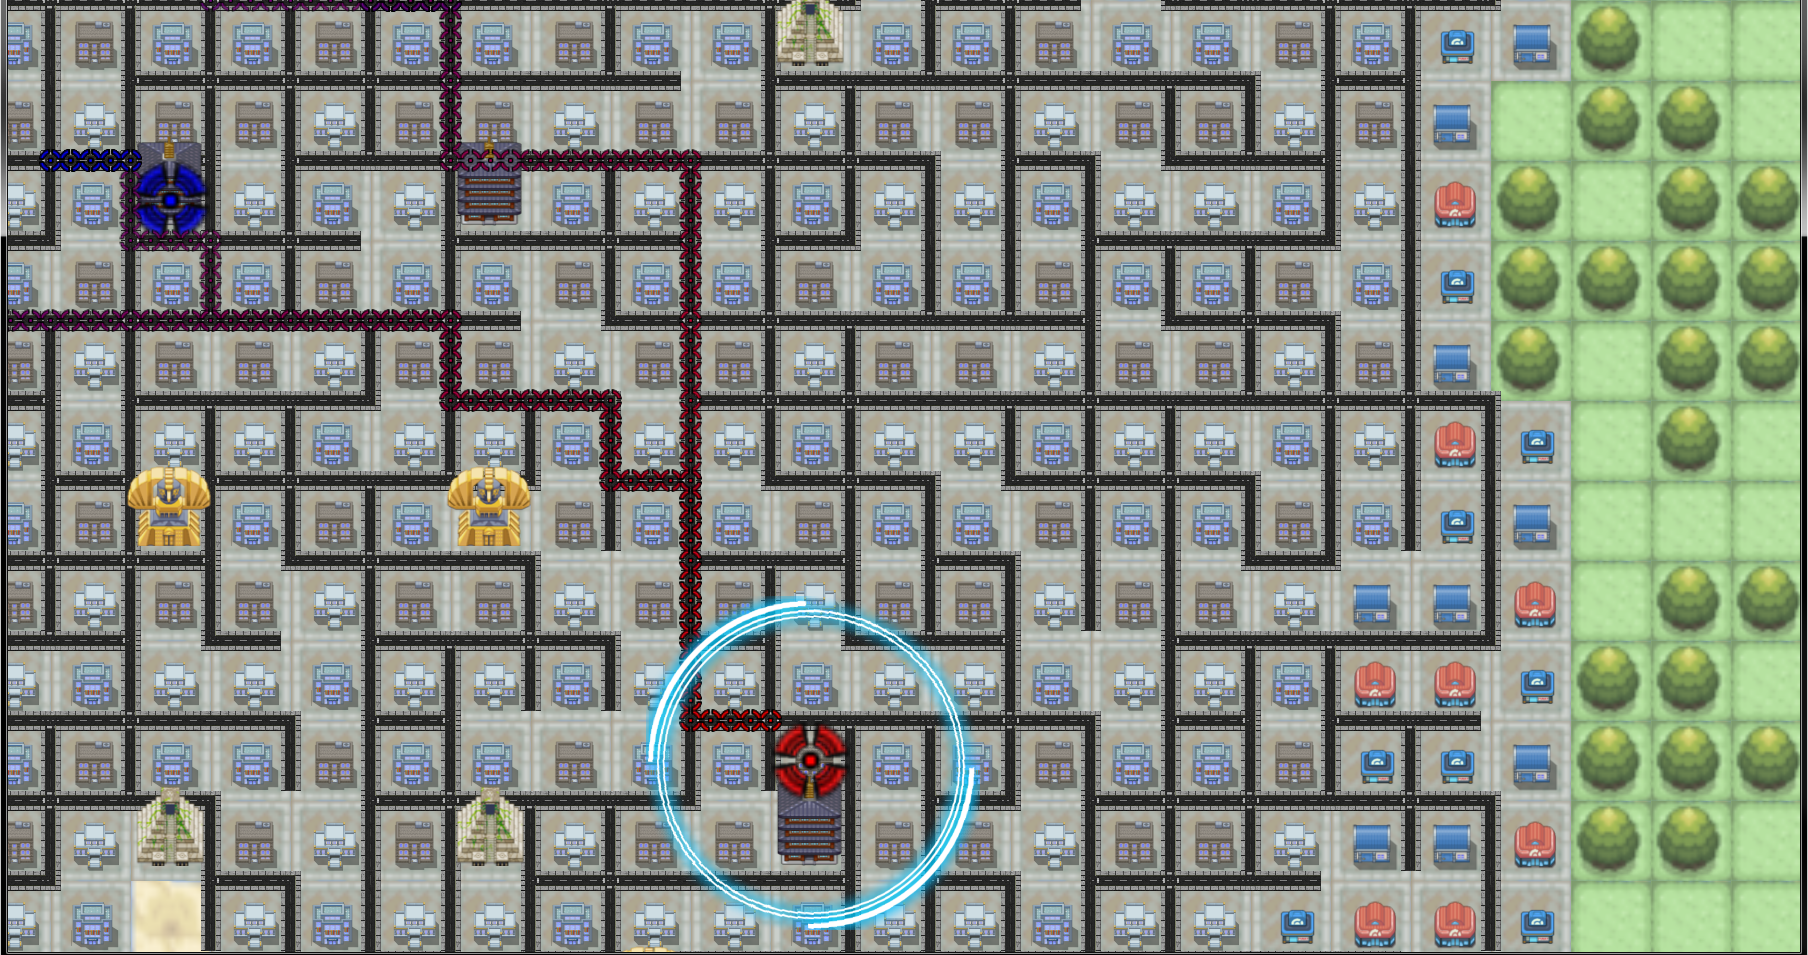
\includegraphics[scale=0.2]{img/exercise4}
\caption{Exercise 3.2 result}
\label{img:Ex3-2}
\end{figure}
\newpage
\printindex


\end{document}
